We propose a techniques to extract and represent the work history and the dependencies among artifacts. The process is depicted in \Cref{fig:visualization-process} and consists of three successive steps towards extracting hidden work dependencies from \gls{vcs} event data. The method works under the following assumptions.

\begin{itemize}
\item [A1:] {\bf Meaningful file tree structure.} The file tree structure in a project represents the structure of work of the project participants.
\item [A2:] {\bf Frequent commits.} Commits to the VCS are regularly performed.  
\item [A3:] {\bf Meaningful comments.} The comments included by project participant when commiting their work represent the changes done to the file being commit.
\end{itemize}

\begin{figure}[h]
\centering
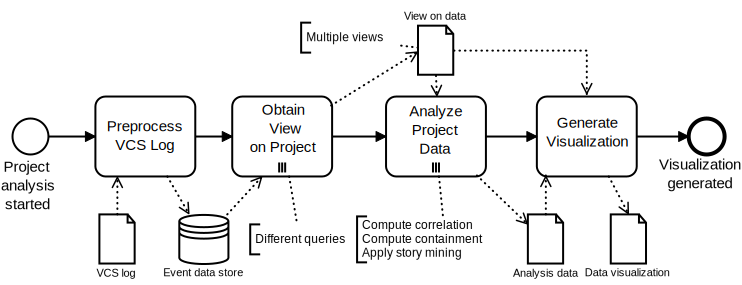
\includegraphics[width=.8\textwidth]{figures/visualization-process}
\caption[Generation of a process visualization from VCS logs]{Generation of a process visualization from VCS logs}
\label{fig:visualization-process}
\end{figure}

The first step of the approach is the preprocessing of the \gls{vcs} log received as input. The main goal of this phase is generate a set of events and store them into a database. Second, we obtain different views on the stored events. In particular, we are interested in observing
\begin{inparaenum}[\itshape i)]
	\item all the commits that affected the files over time;
	\item the amount of change brought by the commits to the files; and
	\item the users who issued such commits.
\end{inparaenum}
The third phase is responsible for considering the different perspectives defined by the project manager and through the generated views extract the necessary knowledge. The last phase is responsible for providing the visualization combining the different perspectives considered. In the following, we detail the formal concepts and the algorithm of our technique.

%\subsubsection{Preprocessing VCS Logs.}
%Version control system logs hold rich information about the artifacts and their evolution. Therefore, our process starts by extracting the elements \emph{Artifact}, \emph{Commit} and \emph{Event} from the log.
%
%First, the tree file is analyzed so the \emph{Parent} relation is defined. For that, the artifacts names appearing in the log are used. They provide the whole path from the root file until the leave file, which is the artifact in question. Thus, a parser can analyses the path and create the relation between the files. For instance, suppose we have the artifact \texttt{running example/software/model.java}. Three files are observed from this name: $f_1 = running \quad example$, $f_2 = software$ and $f_3 = model.java$. The following pairs will be included in the \emph{Parent} relation $\{(f_1,f_2),(f_2,f_3)\}$. 
%%are in the same containment if they share a common prefix that is maximal, i.e. they differ only by the name. For example, the files 
%%and \texttt{running example/software/test.java} . belong to the same containment, whereas the files  \texttt{running example/software/model.java} and \texttt{README.md} belong to two different containments. Note that containments can be contained in other containments, therefore every two files with eventually belong to the same containment. 
%
%Second, artifacts are extracted, as specified in Definition \ref{def_artifact}. Then the commits, following Definition \ref{def_commit}, are extracted. At last, the VCS raw log is transformed into a list of events for the extracted artifacts and commits, as specified in Definition \ref{def_event}. This step is easily done by replicating the information on commit level to be contained in the events. The amount of change is determined analyzing the attribute Diff of the VCS log. For instance, commit ID 2 in Table \ref{tab:vcs-log-data} indicates a commit with amount of change equals 3. The output of this phase is a set of events $E$, a set of artifacts $A$ and a set of commits $Com$.
%
%\subsubsection{Obtain View on Project.}
%The main goal of this phase is to extract the data that will be analyzed. The focus of this paper is in the artifacts, therefore the views generated gather information about events related to artifacts.  
%
%The project manager must determine the level of detail for the analyzes, thus, specifying the time windows. Input parameters of this phase are the interval of analysis ($ia$) and the time window for aggregation ($tw_{agg}$). Considering the specified $tw_{agg}$, the events generated in the previous phase are aggregated. For each artifact in a particular aggregate time an \emph{Aggregate Event} is generated as defined in Definition \ref{def_aggregateEvent}.
%
%\subsubsection{Analyze project data.}
%In this phase, the project is analyzed considering the different perspectives the project manager is interested in. In this paper, we considered three perspectives: dependency between artifacts, containments and artifact evolution.
%
%\paragraph{Dependency.} As stated in \Cref{def_dependency}, a dependency between two artifacts exists if both artifacts require a similar effort to be maintained, i.e. if they have a similar behavior considering the amount of changes.  The amount of change of an artifact over time defines  a time series. Therefore, for each artifact its aggregate events are analyzed in order to extract the amount of change for each aggregated time towards defining a time series for this artifact. 
%
%Let $AE$ be the set of aggregate events within $ia$. We build the time series for the \emph{i}-th artifact, namely $X_{f_i} = \lbrace (t, c) ~|~ e_a \in AE,~ t = ats(e_a),~ c = aac(e_a),~ f(e_a) = {f_i} \rbrace $. 
%
%%\todo[inline]{
%%Dependencies are obtained from the aggregated events. Considering the time window $tw$ and the aggregated event set in that time window ($AE_{tw}$), %$AE' = \lbrace e~|~ e \in AE,~ ts(e) \in tw \rbrace$,
%%we build the time series for the \emph{i}-th artifact, namely $X_{f_i} = \lbrace (t, c) ~|~ e_a \in AE_{tw},~ t = ats(e_a),~ t \in tw,~ c = aac(e_a),~ f(e_a) = {f_i} \rbrace $. As a result, the dependency between \emph{i}-th and the \emph{j}-th artifact is the correlation across time series $\sigma(i,j) = {corr(X_i, X_j)}$.
%%}
%
%After the time serie for each artifact is defined, the correlation function is used to calculate the correlation between the two time series. Considering artifacts $f_i$ and $f_j$ and the time series correspondent $X_{f_i}$ and $X_{f_j}$, $\sigma(f_i,f_j) = {corr(X_{f_i}, X_{f_j})}$ is the correlation value found when applying correlation function $corr$.
%
%If $\sigma(f_i,f_j)$ overcomes a threshold defined by the project manager (input parameter of this phase), then a dependency between the correspondent artifacts is established. The strength of the dependency is defined by $\sigma(f_i,f_j)$. 
%
%\paragraph{Containments.}
%For the containments extraction, the $Parent$ relation is analyzed and the set $C$ of containments defined.
%Containments reflect the hierarchical nature of the file structure in a repository. That is, \emph{composite containments} can be recursively decomposed into smaller containments until an \emph{atomic containment} is reached, following the tree structure of the file system top down. Conversely, from navigating the file structure bottom up, containments can be part of other containments until the root containment is reached. 
%
%
%\paragraph{Artifact evolution.}
%%For the artifact evolution definition, we propose to apply story mining techniques as follows.
%
%%\label{subsec:story-mining}

In a software development scenario, project participants add, remove, modify and perform several different operations in an artifact and store these changes in a shared repository (such as GitHub or Subversion). Different participants may change an artifact, and therefore it is a collaborative work towards a final product. Moreover, they can add comments when committing changes to an artifact bringing insights of the working process performed in this artifact.

We argue that these comments 
%form the textual elements is a kind of story being told, with additional elements such as location (the specific folder and files being manipulated at the broader view of a Project folder tree map) and the timestamp of their specific operation. The comments text and the additional elements
follow a similar structure of the story applied at the Story Mining method  \cite{Goncalves2011} , i.e., the comments provided by the different participants build the story about the work being done in the particular artifact. Moreover, additional elements such as time of the commit and the project participant responsible for the changes provide extra information that can be used to represent the artifact evolution. Therefore, in this research we use story mining to build a process which represents the artifact evolution. The input of the story mining is a set artifact stories, where the story of the \emph{i}-th artifact is obtained from the set $AE$ of aggregated events as $ story({f_i}) = \lbrace {m ~|~ a_e \in AE,~ f(a_e) = f_i,~ ak(a_e)=m} \rbrace$.


%several distinct visualizations from these stories to represent the software process elements, thus depicting critical viewpoints for the participants.
For instance, consider information about $4$ aggregate events related to a specific artifact as depicted in \Cref{table:ExampleOfComments}:

\begin{table}[!h]
	\caption{Comments made by project participants in four different times when committing changes performed in a artifact.}
	\label{table:ExampleOfComments}
\begin{center}
\begin{tabular}{|c|c|l|}
Time & Project Participant & Comment\\\hline
$ats_1$ & $au_1$ & Add requirements file. \\
$ats_2$ & $au_2$ &Update requirements.\\
$ats_3$ & $au_2$ &Modify requirements.\\
$ats_4$ & $au_2$ &Specify solved time for problem.\\
\end{tabular}
\end{center}
  
\end{table}

Using the story mining approach we are able to find the process activities. Then, considering the time of each commit, a workflow is created. Moreover, we associated the participant responsible for the work as the one that committed the changes. The final process discovered for the illustrative example is depicted in Figure \ref{fig:ExampleOfWorkingProcess}.

\begin{figure}[!h]
	\centering
  
\includegraphics[width=.9\linewidth]{ProcessExample}
  \caption{Working process generated from the set of comments depicted in Table
  \label{fig:ExampleOfWorkingProcess} \ref{table:ExampleOfComments}. The color images represent the user responsible for the commit.}
\end{figure}




 %\hfill\\
%1. Compute correlation - dependency
%2. Compute containments 
%3. Apply story mining to obtain the process  - artifact evolution \\\hfill

%\subsubsection{Generate visualization.}
%%The approach is flexible making possible to generate different visualizations 
%In this section, we define the graphical elements of the visualization and their semantic. 
%
%%\input{table/visual-symbols}
%\paragraph{Project Participant.}
%%\todo[inline]{Task was not defined before. I think in our case workload will be in how many changes the project participant is involved within a period of time. I change to this idea. See what do you think. \\[2pt] I also consider project participant instead of resource following what was defined in section II.A. But I am ok with both. We just need to decide and change the whole paper. \\[2pt] The symbols have different faces and the semantic was not provided. I know they align with the color, but I think it is better to have the same face (not all people with high workload are sad or with low workload are happy). On the other hand, we lost the representation of a participant in the process, i.e. we are not able to visualize how many different participant worked in the same process (artifact). If we are still interested in that, I suggest to leave the faces as symbolizing the workload and the colors to symbolize different participants}
%
%Project Participants are displayed through a face symbol with its identification in the top, as depicted in  \Cref{fig:resources}. We use a color code to denote their level of workload, i.e. in how many changes the project participant is involved in the project within $ia$. \emph{Red}, \emph{yellow} and \emph{green} color indicate \emph{high}, \emph{medium} and \emph{low} project workload respectively. The project workload for a project participant ($wl_u$) is computed from the set of events in which the project participant was responsible for the change within $ia$, i.e. $wl_u(t_1,t_2) = |\lbrace e \in E ~|~  u(e)= u, t_1 \leq ts(e) \leq t_2 \rbrace|$, where $ia=[t_1 , t_2]$. These interval of analysis can be fine tuned to visualize the project participant occupancy over time. 
%
%%\begin{figure}[h]
%%	\centering
%%	\begin{subfigure}{.3\linewidth}
%%		\centering
%%		\begin{tikzpicture}[scale=.2]
%%		\node[text width=3cm] at (2,2.3) {resource};
%%		
%%		\filldraw [color=black, fill=green!50] (0,0) circle (2);
%%		\filldraw [color=black, fill=white] (-0.5,.6) ellipse (0.2 and 0.6);
%%		\filldraw [color=black, fill=white] (0.5,.6) ellipse (0.2 and 0.6);
%%		\filldraw [color=black, fill=black] (-0.5,.4) ellipse (0.2 and 0.3);
%%		\filldraw [color=black, fill=black] (0.5,.4) ellipse (0.2 and 0.3);
%%		\draw  (-1,-0.5) .. controls (-0.5,-1) and (0.5,-1) .. (1,-0.5);
%%		\draw  (-1,-0.5) .. controls (-0.5,-1.3) and (0.5,-1.3) .. (1,-0.5);
%%		\fill[fill=white, draw=black, opacity=1] (-1,-0.5) .. controls (-0.5,-1) and (0.5,-1) .. (1,-0.5) .. controls (0.5,-1.3) and (-0.5,-1.3) .. (-1,-0.5) --cycle;
%%		\end{tikzpicture}
%%		%		
\includegraphics[width=.3\linewidth]{figures/visualization-elements/green-face}
%%		\caption{}
%%		\label{fig:green}
%%	\end{subfigure}%
%%	\begin{subfigure}{.3\linewidth}
%%		\centering
%%		%		
\includegraphics[width=.3\linewidth]{figures/visualization-elements/yellow-face}
%%		\begin{tikzpicture}[scale=.2]
%%		\filldraw [color=black, fill=yellow!50] (0,0) circle (2);
%%		\filldraw [color=black, fill=white] (-0.5,.6) ellipse (0.2 and 0.6);
%%		\filldraw [color=black, fill=white] (0.5,.6) ellipse (0.2 and 0.6);
%%		\filldraw [color=black, fill=black] (-0.5,.4) ellipse (0.2 and 0.3);
%%		\filldraw [color=black, fill=black] (0.5,.4) ellipse (0.2 and 0.3);
%%		%mouth
%%		%		\draw  (-1,-0.6) .. controls (-0.5,-1) and (0.5,-1) .. (1,-0.5);
%%		%	\draw  (-1,-0.5) .. controls (-0.5,-1.3) and (0.5,-1.3) .. (1,-0.5);
%%		\fill[fill=white, draw=black, opacity=1] (-1,-0.7) .. controls (-0.5,-0.8) and (0.5,-0.8) .. (1,-0.7) .. controls (0.5,-1) and (-0.5,-1) .. (-1,-0.7) --cycle;
%%		\end{tikzpicture}
%%		\caption{}
%%		\label{fig:yellow}
%%	\end{subfigure}%
%%	\begin{subfigure}{.3\linewidth}
%%		\centering
%%		%		\includegraphics[width=.3\linewidth]{figures/visualization-elements/red-face}
%%		\begin{tikzpicture}[scale=.2]
%%		\filldraw [color=black, fill=red!60] (0,0) circle (2);
%%		\filldraw [color=black, fill=white] (-0.5,.6) ellipse (0.2 and 0.6);
%%		\filldraw [color=black, fill=white] (0.5,.6) ellipse (0.2 and 0.6);
%%		\filldraw [color=black, fill=black] (-0.5,.4) ellipse (0.2 and 0.3);
%%		\filldraw [color=black, fill=black] (0.5,.4) ellipse (0.2 and 0.3);
%%		%			\draw  (-1,-0.5) .. controls (-0.5,-1) and (0.5,-1) .. (1,-0.5);
%%		%		\draw  (-1,-0.5) .. controls (-0.5,-1.3) and (0.5,-1.3) .. (1,-0.5);
%%		\fill[fill=white, draw=black, opacity=1] (-1,-1) .. controls (-0.5,-0.5) and (0.5,-0.5) .. (1,-1) .. controls (0.5,-0.8) and (-0.5,-0.8) .. (-1,-1) --cycle;
%%		\end{tikzpicture}
%%		\caption{}
%%		\label{fig:red}
%%	\end{subfigure}
%%	\caption{Project Participant symbols. Color codes represent the status of their workload within a period of time.}
%%	\label{fig:resources}
%%\end{figure}
%
%
%%\begin{figure}[h]
%%	\centering
%%		\begin{tikzpicture}[scale=.2]
%%		\node[] at (0,3.5) {\textit{participant}};
%%		\filldraw [color=black, fill=white!50] (0,0) circle (2);
%%		\filldraw [color=black, fill=white] (-0.5,.6) ellipse (0.2 and 0.6);
%%		\filldraw [color=black, fill=white] (0.5,.6) ellipse (0.2 and 0.6);
%%		\filldraw [color=black, fill=black] (-0.5,.4) ellipse (0.2 and 0.3);
%%		\filldraw [color=black, fill=black] (0.5,.4) ellipse (0.2 and 0.3);
%%		%mouth
%%		%		\draw  (-1,-0.6) .. controls (-0.5,-1) and (0.5,-1) .. (1,-0.5);
%%		%	\draw  (-1,-0.5) .. controls (-0.5,-1.3) and (0.5,-1.3) .. (1,-0.5);
%%		\fill[fill=white, draw=black, opacity=1] (-1,-0.7) .. controls (-0.5,-0.8) and (0.5,-0.8) .. (1,-0.7) .. controls (0.5,-1) and (-0.5,-1) .. (-1,-0.7) --cycle;
%%		\end{tikzpicture}
%%	\caption{Project Participant symbol. The workload within a period of time is color coded.} 
%%	\label{fig:resources}
%%\end{figure}
%
%
%
%\paragraph{Dependency.}
%A dependency between two artifacts is represented by a line that connects their atomic containments. We label dependencies with a number  $\sigma \in \Re$, which indicates the strength of the dependency among the two artifacts. \Cref{fig:dependency} illustrate the notation for dependencies.
%
%%\begin{figure}[h]
%%	\centering
%%	%	\includegraphics[width=0.7\linewidth]{figures/visualization-elements/dependency}
%%	\begin{tikzpicture}[scale=.5]
%%	\draw[thick] (-2,0) -- node[above,thick] {$\sigma$} ++(4,0);
%%	\end{tikzpicture}
%%	\caption{Dependency with strength $\sigma$}
%%	\label{fig:dependency}
%%\end{figure}
%
%\paragraph{Artifact evolution.}
%
%The artifact evolution is a process under which the artifact changes step by step towards a final state reached eventually in the project (e.g. a documentation file reaches his final state when the documentation is complete and no edits are made to that version of document anymore). Thus, we chose the \gls{bpmn} to represent this process. 
%
%\Cref{fig:process} depicts an example of a process learned considering a story with two aggregated comments, thus a process with two sequential activities \emph{a} and \emph{b}, modeled in \gls{bpmn}. 
%
%%\tikzstyle{startstop} = [rectangle, rounded corners, minimum width=1.5cm, minimum height=1cm,text centered, draw=black, fill=white!30]
%%\tikzstyle{arrow} = [thick,->,-latex]
%%\tikzstyle{event} = [circle,scale=.5, minimum width=1cm, minimum height=1cm,draw,fill=white]
%%\tikzstyle{end event} = [event,ultra thick]
%%
%%\begin{figure}[h]
%%	\centering
%%	%
\includegraphics[width=0.7\linewidth]{figures/visualization-elements/process}
%%	\begin{tikzpicture}[scale=.3]
%%	\begin{scope}[auto, every node/.style={draw,circle},node distance=.2cm]
%%	\node (start) [event] {};
%%	\node (add) [startstop, right of=start, xshift=1.3cm] {a};
%%	\node (fix) [startstop, right of=add, xshift=1.9cm] {b};
%%	\node (end) [end event, right of=fix, xshift=2.8cm] {};
%%	\draw [arrow]  (start) -- (add);
%%	\draw [arrow]  (add) -- (fix);
%%	\draw [arrow]  (fix) -- (end);
%%	\end{scope}
%%	\end{tikzpicture}
%%	\caption{Process representing an artifact evolution using \gls{bpmn}.}
%%	\label{fig:process}
%%\end{figure}
%
%
%\paragraph{Containment.} 
%A containment is represented with a rectangle. 
%We overload the semantic of rectangle used to represent the containment with a time concept. The position of the \emph{atomic containments} is shifted within the boundaries of their parent containments according to the first timestamp of the artifact history. For example, given two \emph{atomic containments} $C_1\{f_i\}$, $C_2\{f_j\} \subseteq C$, and let $AE_i, AE_j \subseteq AE$ be the sets of aggregated events that affected these artifacts, respectively. Then $C_1$ is shifted left with respect to $C_2$ if $min\{ats(e) | e \in AE_i\} < min\{ats(e') | e' \in AE_j\}$. \Cref{fig:containment} illustrates this example.
%
%%\begin{figure}[h]
%%\centering
%%%\includegraphics[width=0.7\linewidth]{figures/visualization-elements/containment}
%%\usetikzlibrary{
%%	shapes.geometric,
%%	positioning,
%%	fit,
%%	calc
%%}
%%\begin{tikzpicture}
%%	\draw[thick] (0,0)rectangle (4,2) node[pos=.85] {$C_3$};
%%	\draw[thick] (1.1,1.1) rectangle (2.2,1.6) node[midway] {$C_1$}; 
%%	\draw[thick] (2.1,0.1) rectangle (3.2,0.6) node[midway] {$C_2$};
%%\end{tikzpicture}
%%\caption{A containment $C_3$ composed of two atomic containments $C_1$, $C_2$. $C_1$ is shifted more left wrt $C_2$ as its contained artifacts were affected by changes earlier.}
%%\label{fig:containment}
%%\end{figure}
%
%\begin{figure}
%	\centering
%	\begin{subfigure}[t]{.5\textwidth}
%		\centering
%		\begin{tikzpicture}[scale=.2]
%		\node[] at (0,3.5) {\textit{participant}};
%		\filldraw [color=black, fill=white!50] (0,0) circle (2);
%		\filldraw [color=black, fill=white] (-0.5,.6) ellipse (0.2 and 0.6);
%		\filldraw [color=black, fill=white] (0.5,.6) ellipse (0.2 and 0.6);
%		\filldraw [color=black, fill=black] (-0.5,.4) ellipse (0.2 and 0.3);
%		\filldraw [color=black, fill=black] (0.5,.4) ellipse (0.2 and 0.3);
%		%mouth
%		%		\draw  (-1,-0.6) .. controls (-0.5,-1) and (0.5,-1) .. (1,-0.5);
%		%	\draw  (-1,-0.5) .. controls (-0.5,-1.3) and (0.5,-1.3) .. (1,-0.5);
%		\fill[fill=white, draw=black, opacity=1] (-1,-0.7) .. controls (-0.5,-0.8) and (0.5,-0.8) .. (1,-0.7) .. controls (0.5,-1) and (-0.5,-1) .. (-1,-0.7) --cycle;
%		\end{tikzpicture}
%		\caption{Project Participant symbol. The workload within a period of time is color coded.} 
%		\label{fig:resources}
%	\end{subfigure}~
%	\begin{subfigure}[t]{.5\textwidth}
%		\centering
%		%	\includegraphics[width=0.7\linewidth]{figures/visualization-elements/dependency}
%		\begin{tikzpicture}[scale=.5]
%		\draw[thick] (-2,0) -- node[above,thick] {$\sigma$} ++(4,0);
%		\end{tikzpicture}
%		\caption{Dependency with strength $\sigma$}
%		\label{fig:dependency}
%	\end{subfigure}\\
%	\begin{subfigure}[t]{.5\textwidth}
%		\tikzstyle{startstop} = [rectangle, rounded corners, minimum width=1.1cm, minimum height=.6cm,text centered, draw=black, fill=white!30]
%		\tikzstyle{arrow} = [thick,->,-latex]
%		\tikzstyle{event} = [circle,scale=.7, minimum width=.5cm, minimum height=.5cm,draw,fill=white]
%		\tikzstyle{end event} = [event,ultra thick]
%		%		\begin{figure}[h]
%		\centering
%		%
\includegraphics[width=0.7\linewidth]{figures/visualization-elements/process}
%		\begin{tikzpicture}
%		\begin{scope}[auto, every node/.style={draw,circle},node distance=.05cm]
%		\node (start) [event] {};
%		\node (add) [startstop, right of=start, xshift=1cm] {a};
%		\node (fix) [startstop, right of=add, xshift=1.5cm] {b};
%		\node (end) [end event, right of=fix, xshift=1.6cm] {};
%		\draw [arrow]  (start) -- (add);
%		\draw [arrow]  (add) -- (fix);
%		\draw [arrow]  (fix) -- (end);
%		\end{scope}
%		\end{tikzpicture}
%		\caption{Process representing an artifact evolution using \gls{bpmn}.}
%		\label{fig:process}
%		%		\end{figure}
%	\end{subfigure}~~
%	\begin{subfigure}[t]{.45\textwidth}
%		\centering
%		%\includegraphics[width=0.7\linewidth]{figures/visualization-elements/containment}
%		\usetikzlibrary{
%			shapes.geometric,
%			positioning,
%			fit,
%			calc
%		}
%		\begin{tikzpicture}[scale=.99]
%		\draw[thick] (0,0)rectangle (4,2) node[pos=.85] {$C_3$};
%		\draw[thick] (1.1,1.1) rectangle (2.2,1.6) node[midway] {$C_1$}; 
%		\draw[thick] (2.1,0.1) rectangle (3.2,0.6) node[midway] {$C_2$};
%		\end{tikzpicture}
%		\caption{A containment $C_3$ composed of two atomic containments $C_1$, $C_2$. $C_1$ is shifted more left wrt $C_2$ as its contained artifacts were affected by changes earlier.}
%		\label{fig:containment}
%	\end{subfigure}
%	\caption{Graphic elements used to represent the defined concepts of project participant, work dependency, artifact evolution and containment.}
%\end{figure}
%
%\paragraph{Composing the visualization.}
%
%The layout rules to compose the visualization are the following. 
%\begin{inparaenum}[\itshape (i)]
%	\item Every element is within a containment, excluding the root;
%	\item Project participants responsible for the change are placed over \gls{bpmn} activities;
%	\item Artifact evolution is within an atomic containment;
%	\item Dependencies connect atomic containments, showing the strength of correlations between the belonging artifacts evolutions.
%\end{inparaenum}
%\Cref{fig:all-elements-together} shows the correct composition of the presented visual elements.
%
%\begin{figure}
%\centering
%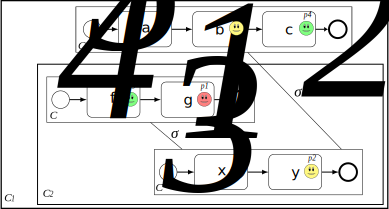
\includegraphics[width=.6\linewidth]{figures/visualization-elements/al-elements-together}
%\caption{Composition of the graphic elements into five containments, of which two are composite.}
%\label{fig:all-elements-together}
%\end{figure}

